\documentclass[conference]{IEEEtran}
\IEEEoverridecommandlockouts
% The preceding line is only needed to identify funding in the first footnote. If that is unneeded, please comment it out.
\usepackage{cite}
\usepackage{amsmath,amssymb,amsfonts}
\usepackage{algorithmic}
\usepackage{graphicx}
\usepackage{textcomp}
\usepackage{xcolor}
\def\BibTeX{{\rm B\kern-.05em{\sc i\kern-.025em b}\kern-.08em
    T\kern-.1667em\lower.7ex\hbox{E}\kern-.125emX}}
\begin{document}

\title{Systems of Digital Twins and Physical Systems: Interoperability, Decentralization, and Mobility in Robotic Applications}

\author{\IEEEauthorblockN{Felix Girke}
\IEEEauthorblockA{\textit{Dept. of Comp. Science \& Engineering} \\
\textit{Frankfurt University of Applied Sciences}\\
Frankfurt a.M., Germany \\
https://orcid.org/0009-0004-3967-6750}
\and
\IEEEauthorblockN{René Harmann}
\IEEEauthorblockA{\textit{Dept. of Comp. Science \& Engineering} \\
\textit{Frankfurt University of Applied Sciences}\\
Frankfurt a.M., Germany \\
rene.harmann@fb2.fra-uas.de}
\and
\IEEEauthorblockN{Eric Guiffo Kaigom}
\IEEEauthorblockA{\textit{Dept. of Comp. Science \& Engineering} \\
\textit{Frankfurt University of Applied Sciences}\\
Frankfurt a.M., Germany \\
kaigom@fb2.fra-uas.de}
}

\maketitle

\begin{abstract}
Whereas digital twins are receiving an increasing
attention, their implementation has been predominated by mono-
lithic and static solutions. A resulting issue is the lack of a
modular integration and seamless interplay of digital twins when
it comes to adapt and support varying industrial and societal
applications. Another drawback arises from limited services that
digital twins can provide as the physical system is extended
with new components and/or separated from constituting parts,
giving rise to a metamorphosic system of systems. Furthermore,
the respective mobility of physical systems and citizens assumed
to interact with them via their digital surrogates is hardly
transformed into industrial and societal opportunities, such as
a pervasive and itinerant human-robot-interaction ($\pi$-HRC).
Within the scope of our Metarobotics framework that propels
$\pi$-HRC, we address these challenges by leveraging on the OPC-UA standard to develop portable data connectors that move
with and give access to the data source, which is the associated
physical system. Our Raspberry-Pi driven connector encapsulates
a digital twin of the corresponding system and its offered services
to capture the loose coupling and decentralization of systems
and systems even remotely and in motion. Each data connector
semantically interoperates with any OPC-UA capable system
and device via wireless communication. This opens up new
opportunities for different monitoring (and control) modalities
of large scale systems whose physical or/and virtual constituting
subsystems are distributed across distinct geographical locations
in the industrial and societal realm. We apply our framework
to a mobile multi-arm robotic system with edge-computing
capabilities and demonstrate the performance of its monitoring
functionality from the cabin of a moving train in city traffics
in practice. We provide experimental measurements results and
highlight the usefulness and effectiveness of our approach.
% To solve the problem of different interfaces for different robots a data connector is developed.
% It creates a interoperable, decentralized network for a robot system using the Open Platform Communication Unified Architecture (OPC-UA) standard.
% Using this network a flexible digital twin is created in Isaac Sim to visualize the data of the robot system.
% To monitor the robot system from everywhere the possibility of an remote access to the data connectors is set up.
\end{abstract}

\begin{IEEEkeywords}
Robotics, Digital Twins, System of Systems, Industry 4.0, Industry 5.0, Society 5.0, Human-Robot-Interaction
% OPC-UA, interoperable, decentralized, digital Twin, Isaac Sim, remote access
\end{IEEEkeywords}

\section{Introduction}
Most robot manufacturers develop their own framework to monitor, plan, and control their robots. Challenges arise when trying to assemble a new robotized system of systems composed of multiple single robots from different brands.
In the example  on the lower left hand-side (l.h.s) of Fig. \ref{fig:TitelBild}, two robot arms by Kinova are to be mounted on a Husky mobile robot platform by Clearpath.
\begin{figure}[htbp]
    \centerline{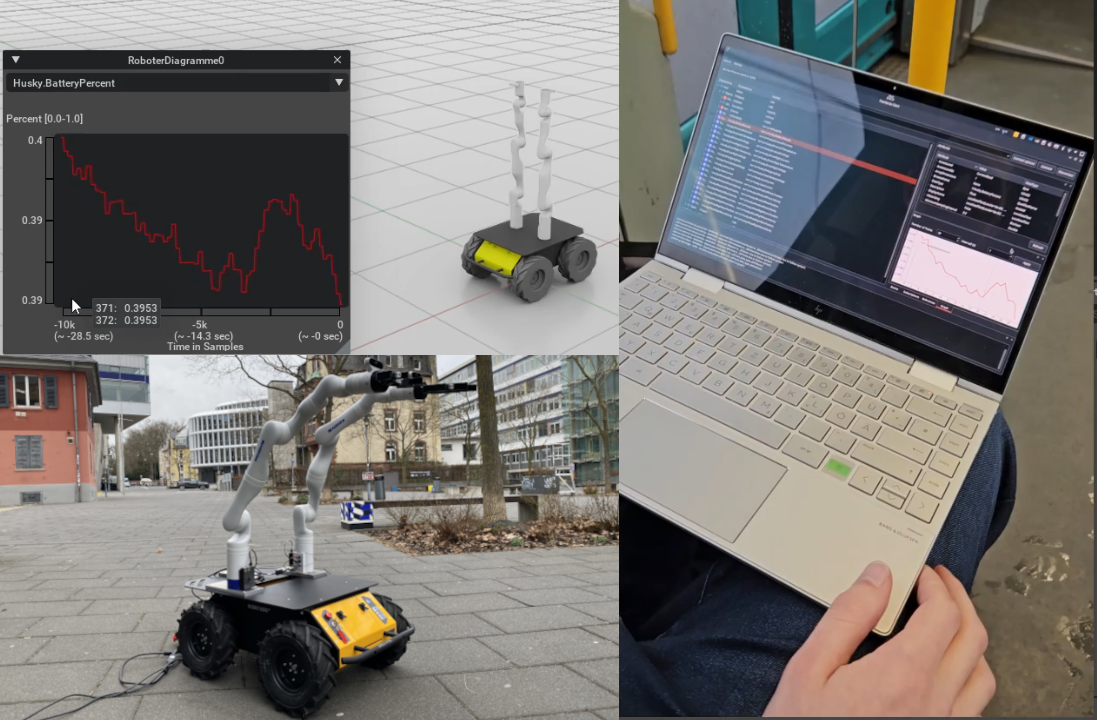
\includegraphics[width=8.9cm]{Pictures/TitelBild.png}}
    \caption{Physical robot system (bottom left) with its digital twin (top left) and remote access (right) to both from the cabin of a moving train in city traffics.}
    \label{fig:TitelBild}
\end{figure}
The Husky, for instance, uses the Robot Operating System (ROS) to communicate internally. By contrast, access is given to both robot arms through the Kortex API by Kinova. New manipulation and logistics capabilities can be yielded by integrating or removing  some of these physical devices (i.e., arm and  base) having heterogeneous programming languages. This can even be done  in a hybrid (i.e., virtual or physical) way   combining real robots with  their digital twins.  Maintenance and reconfiguration goals  to adapt to changing tasks are  use cases \cite{mbakop2023integrated}. It is thus important that these hybrid  single systems  semantically understand each other to exchange information for they reconfigurable and seamless interplay, even \mbox{when they are  at distinct geographical locations.}  

 
To address these challenges, we have developed a data connector (DC) that leverages the Open Platform Communication Unified Architecture (OPC-UA) standard.
A DC acts as a unifying bridge between robot specific languages and any other OPC-UA capable hybrid entity, to which it exposes robot data. Each robot has its own DC, which 
 adds flexibility, since  robot data are not managed by a central server.
Because of this decentralized approach, every client (i.e., entity) can connect only to the DC it needs to. Each DC  communicates via a low-latency 5G wireless network, allowing to remotely aggregate data  from   relevant physical counterparts only,  instead of the whole system. Benefits include the  composability and decomposability of physical and digital robots without data interference and \mbox{from any location, including workplaces in motion.} 
\section{State of the art}
Connecting  different robots together  to form a network has been addressed by different teams.
In \cite{SotaCAN} three robotic arms have been connected using CAN for a cooperative task.
The translation between the robots and the local CAN network is achieved by using a microcontroller for each robot.\\
A similar network was built in \cite{SotaROS}, where ROS is used as a communication protocol.
Unlike the first paper, the robots differ from each other and they all possess native support for ROS. Hence,  there is no need for a translation layer between the robot and the network. To improve the flexibility in  the network proposed in \cite{StoaROStoOPCUA},  interoperability between ROS and  OPC-UA is achieved by integrating them into a local cloud framework. A completely different approach was adopted in \cite{SotaRaconteur} and \cite{SotaFusion}, in which
a middleware was developed to build a network for the different heterogeneous robots.
While the Robot Raconteur software from \cite{SotaRaconteur} is open source, the CorteX software from \cite{SotaFusion} is not.
Furthermore CorteX is built specifically for a robot system working in a Fusion Reactor while Robot Raconteur is an ecosystem for different robots.
% -- Robot Raconteur Middleware for robots (https://ieeexplore.ieee.org/abstract/document/10260569)\\
% -- CorteX, plug and play, distributed system of systems, Fusions Reactor, ähnlich OPC UA aber mit control (https://www.mdpi.com/2218-6581/10/3/108)\\
% -- Interoperability ROS und OPC-UA (https://ieeexplore.ieee.org/abstract/document/9816962)\\
% -- Can Bus, 3 Arme, dezentral, mikocontroller, lokal (https://link.springer.com/chapter/10.1007/978-981-15-5281-6\_30)\\

% --heterogen Robot network, all using ros (https://ieeexplore.ieee.org/abstract/document/9707460)\\
% homogen Robot network peer to peer, find path (https://ieeexplore.ieee.org/document/9196672)\\
\section{Advantages of OPC-UA}
The fourth industrial revolution is about making machines and products "smart" to make decisions and control the manufacturing process on their own \cite{Industry4}.
To make these decisions, robots need to be connected to other machines and resources to get data upon which the decisions are based and made.
Different standards were built to meet this need. Two of the most popular are Message Queuing Telemetry Transport (MQTT) and OPC-UA \cite{CommTechnology}.
Both are built on the Transmission Control Protocol (TCP).
UA is a standard published by the Open Platform Communication Foundation in 2008 and is an "platform independent service-oriented architecture that integrates all the functionality of the individual OPC Classic specifications into one extensible framework" \cite{OPCUA}.
While MQTT is only event driven, OPC-UA, by contrast, features both a Remote Procedure Call (RPC) and   Publish-Subscribe mode \cite{OPCUA} that mitigates polling. 
OPC-UA is not as lightweight as MQTT, but its information model is much more semantics-driven and it outperforms MQTT in many ways \cite{CommunicationCommarison}.
In 2014, the Fraunhofer IOSB has started the open62541 library for C in cooperation with RWTH Aachen and the TU Dresden \cite{open62541}.
Today, this is one of the feature richest open source implementation of the OPC-UA standard \cite{ComparOPCUAPaper}.
Also, there is FreeOpcUa as a very easy-to-use python library.
Its performance might not be as good as the C-library. However, with a powerful PC, it is not the limiting factor and can also be used.
The architecture of OPC-UA as a standard between all DCs, each of them viewed as a server, and entities acting as clients,  makes it helpful to setup a network of decentralized and interoperating robots.
The network might be made up of multiple servers and clients that  talk to servers simultaneously, leading to a dense and understandable information flow. Furthermore, OPC-UA supports  multiple security critical functionalities, including session encryption, message signing, and authentication. \cite{OPCUA}
\section{Development of the data connector}
%Depending on the robot, it might be possible to install software on it.
%If this is the case, there is no need for additional Hardware.
The onboard edge PC of the Husky robot  runs ROS. It is therefore possible to create a ROS package with an OPC-UA server.
For both Kinova robotic arms, on the other hand,  software are hardly installed. As a result, a Raspberry Pi is used as a DC. As such, a DC collects  data from the robot control unit, and makes these data accessible via its built-in OPC-UA server. A Raspberry PI 3B+ is used as hardware for the stand-alone device. This is because of its very versatile nature. It can connect to robots via Ethernet, USB, or various GPIO pins. Furthermore it is powerful enough to host an OPC-UA server and communicate to a robot at the same time.
Because of its small size, it can be mounted directly on e.g. the Kinova robot without self-collision (Fig. \ref{fig:dataConectorPic}).\\

\begin{figure}[t]
    \centerline{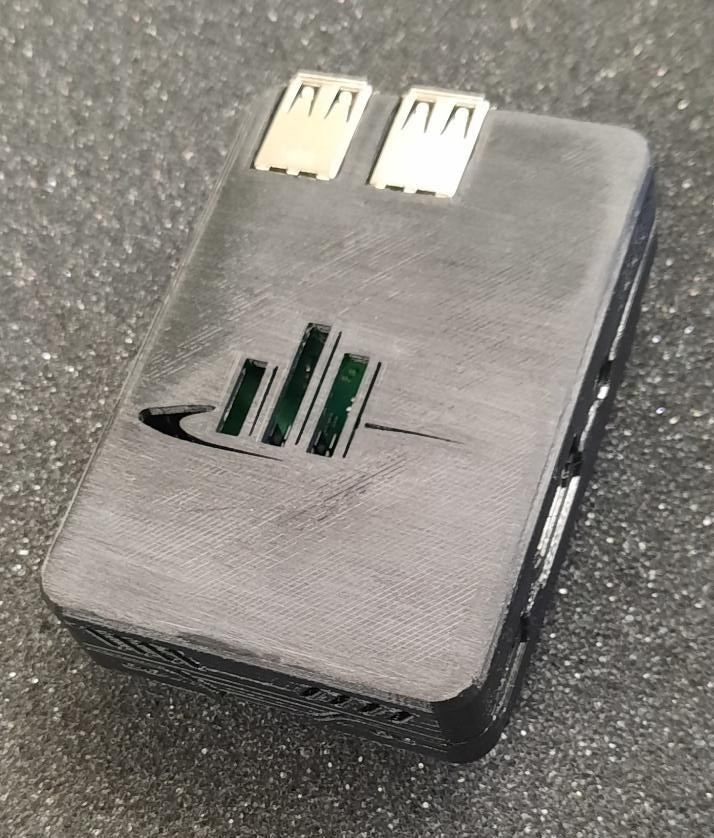
\includegraphics[height=4.9cm]{Pictures/PiGehaeuseVorne.jpeg}\hspace{0.1cm}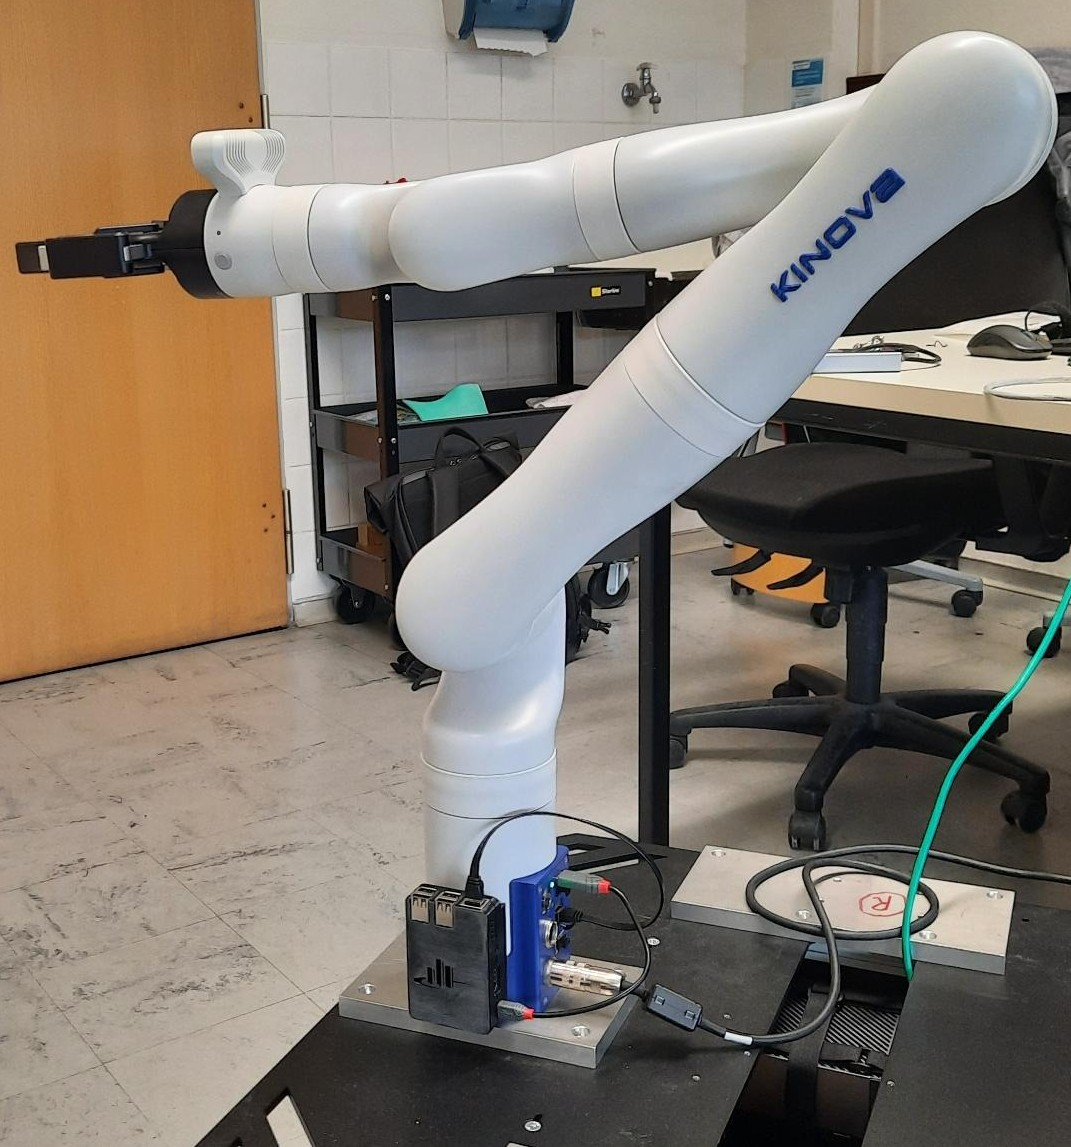
\includegraphics[height=4.9cm]{Pictures/PiAmKinova.jpeg}}
    \caption{The DC (l.h.s) mounted directly on the Kinova robot (r.h.s).}
    \label{fig:dataConectorPic}
\end{figure}

Furthermore, each DC can  be powered by the USB ports of the Kinova robot. No additional power source and expertise are needed, which contributes to Plug and Automate. The structure of the \mbox{DC code is split into three main parts (Fig. \ref{fig:dataConectorStructure}).}

\begin{figure}[b]
    \centerline{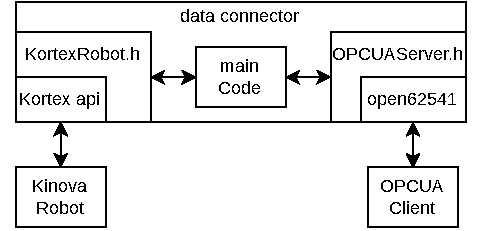
\includegraphics{Pictures/dataConectorStructure.pdf}}
    \caption{Code structure of the data connector.}
    \label{fig:dataConectorStructure}
\end{figure}
The first part is devoted to the communication with the robot via the Kortex API. The second one is the OPC-UA server of the DC with the open62541 library.
The connection to the robot is done using the UDP protocol and  data are requested via the cyclic feedback function of the Kortex API. A reason is that it is a very fast way to collect  data from the robot.
The third and main code part in the middle  starts a thread for the connection to the robot and a thread for the OPC-UA server. It also connects  data from from the robot class to the OPC-UA server class. For this purpose, there is a map defined that connects the function needed to collect  data from the robot to the name of the variable on the OPC-UA server side.
Therefore, variables are intuitively added or removed  from the OPC-UA server by adding or removing an entry from this map. The resulting  system is flexible and versatile. In fact, each DC is not only plug and play capable, but also moveable with any of the Kinova robot arms because they are all using the Kortex API. 
If a DC is to be used with another robot, it is straightforward to add a new connection to the robot and adapt the main code.
It is also possible to prepare the connection protocol for multiple robots from different manufacturers and let the main code detect which robot is \mbox{connected and which protocol is the most appropriate.}

\section{Performance Tests}
To assess how long data takes from the robot to a client, a series of performance tests are conducted.
Tests can be split into two parts. 
First getting  data from the robot to the DC and second collecting  data from the DC to the client.
Each test is made with 5 samples. A single sample is the average speed of the first 1000 data requests.
\subsection{Getting data from the robot}
The Raspberry Pi 3B+ is directly connected to the Kinova robot via an ethernet cable.
With UDP as communication standard, the Raspberry Pi collects  up to 1400 datasets per second from the Kinova robot (Fig. \ref{fig:KortexAPISpeed}).
That is even more than the 1000 datasets per second, that Kinova claims \cite{KortexUDP}. A dataset consists of all  data that the robot has to offer, which are over 50 data points.
If the OPC-UA server is running at the same time on the Raspberry Pi, the frequency is lower, around 1kHz.
If one client is simultaneously requesting data from the OPC-UA server, the frequency is not really affected, but if there are more clients, the frequency begins to drop.

\begin{figure}[htbp]
    \centerline{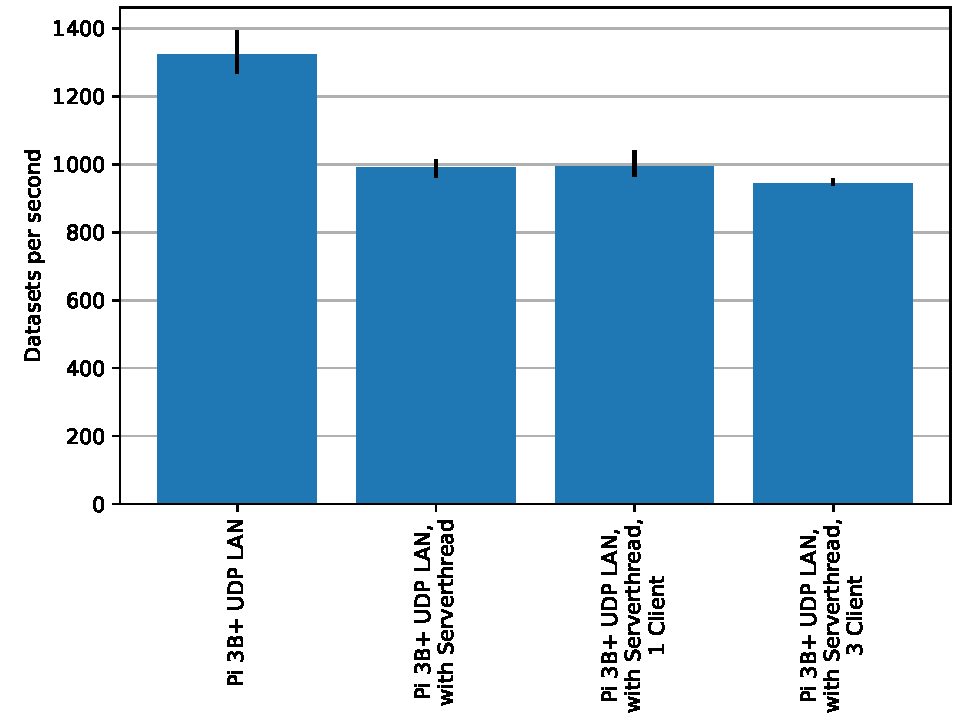
\includegraphics[width=9.1cm]{Pictures/KortexAPISpeed.pdf}}
    \caption{Frequency with which the Raspberry Pi 3B+ can get data from the Kinova arm.}
    \label{fig:KortexAPISpeed}
\end{figure}

\subsection{ Collecting data from the data connector}
To get  data from the DC, two different PCs are used. A midrange Laptop (Intel 11.Gen Core i7-1165G7, Realtek Semiconductor
RTL8152 Fast Ethernet Adapter) and a high end Tower PC (Intel 13.Gen Core i9-13900KF, Realtek Gaming R2.5GbE Family Controller).
The PCs and and DCs are all connected to the same Router (tp-link Archer C80 AC1900 MU-MiMO). In Fig. \ref{fig:OPCUASpeed1D}, different libraries are used for the client to request one value from the DC.
On the Laptop, the C-library open62541 is faster than the python library FreeOpcUa.
\textit{On the Tower PC}, the python library is even faster than the C-library \textit{on the Laptop}.
If these results are compared to the ping between  PCs and DCs (Fig. \ref{fig:PingDiagram}), it can be concluded that the python library on the Tower PC is running close to the actual limit of the network.\\

\begin{figure}[t]
    \centerline{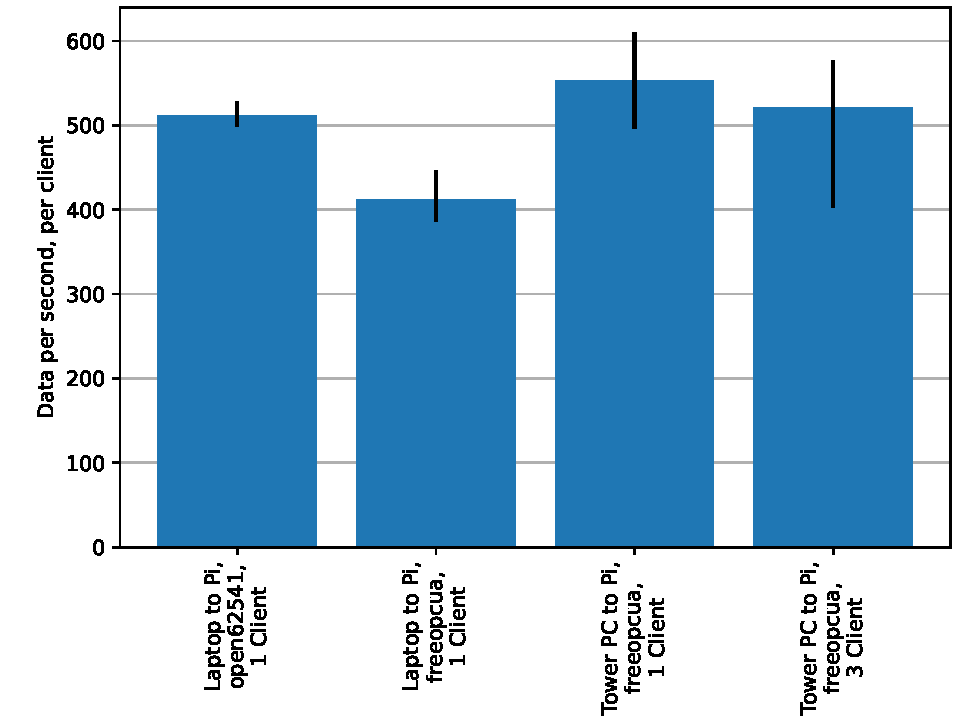
\includegraphics[width=9.1cm]{Pictures/OPCUASpeed1D.pdf}}
    \caption{Frequency with which data can be requested from the OPC-UA server.}
    \label{fig:OPCUASpeed1D}
\end{figure}


\begin{figure}[htbp]
    \centerline{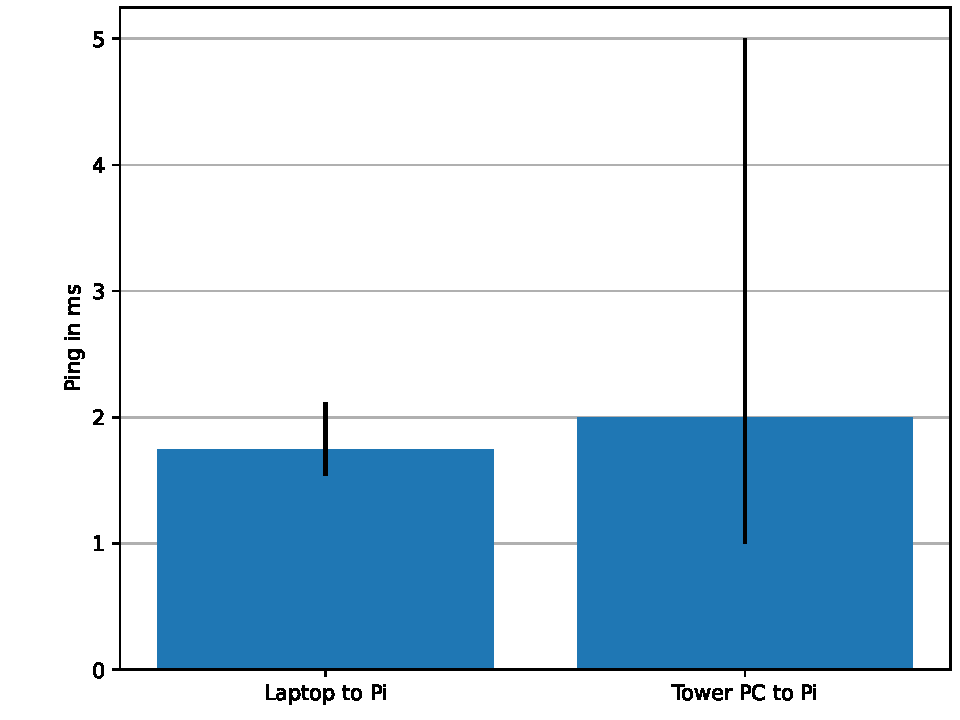
\includegraphics[width=9cm]{Pictures/PingDiagram.pdf}}
    \caption{Ping to the data connector.}
    \label{fig:PingDiagram}
\end{figure}
As multiple clients are started in parallel on the Tower PC, there is a slight decrease in the frequency with which  data can be requested from the DC (Fig. \ref{fig:OPCUASpeed1D}).\\
\begin{figure}[b]
    \centerline{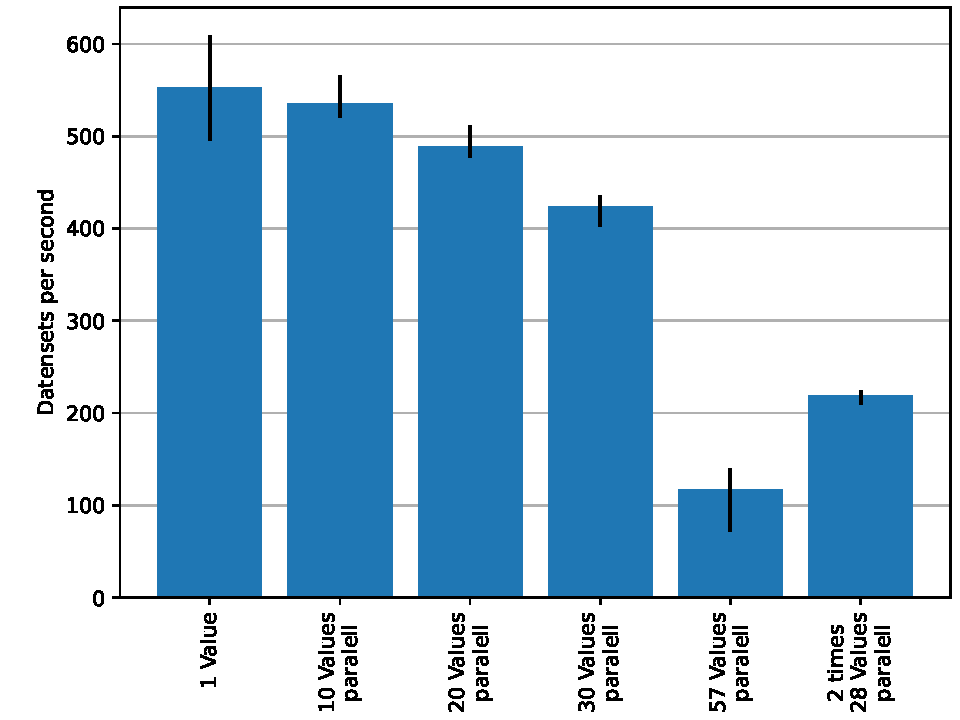
\includegraphics[width=9.1cm]{Pictures/OPCUAMultipleDatenAufEinmal.pdf}}
    \caption{Frequency with which different datasets can be requested from the OPC-UA server.}
    \label{fig:OPCUAMultipleDatenAufEinmal}
\end{figure}
In the final test, (Fig. \ref{fig:OPCUAMultipleDatenAufEinmal}) datasets with different amounts of values are requested from the DC via the Tower PC using the python library.
The difference between 1 value and 10 values in one request is relative small (18 packages), between 10 and 20 values this gap widens (47 packages) and between 20 and 30 it is even bigger (64 packages).
It is clearly not a linear decrease, but also not an exponential one. 
Both the PC and the Raspberry Pi are consuming less than 20\% of the CPU so this is not the bottleneck.
The size of the package gets bigger with every additional value and it seems to be no limit at which the packages are split.
If all 57 values are requested in one package, its size is 2538 bytes.
This length depends mostly upon the name of the values because the longer they are, the bigger the package.
A suitable way to request so many values is in two packages with respectively 28 and 29 values. The frequency is half that of one 30 values package, but this is still nearly two times as fast as requesting all 57 values in one package.
\section{State of Charge of the  battery of the Husky}
Not all data can be directly collected by the OPC-UA server.
For example, the State of Charge (SoC) of the Husky battery is only visible as a four segment display and not numerically available.
The display is probably tuned for a lithium ion battery, so it is  inaccurate for the sealed lead-acid battery (SLA) that is currently powering the mobile Husky robot. It shows only around 50\% SoC with an full battery and, after a short time of usage, it shows 0\% SoC.
To provide a more accurate estimation of the SoC for power monitoring, a ROS package uses the measured current and potential of the battery and publishes an estimation of the SoC tuned for the used SLA battery.
These data are \mbox{also published by the DC OPC-UA server.}
\subsection{Estimating the SoC}
In the user manual of the Husky, Fig. \ref{fig:EndladekuvenSLA} can be found.
\begin{figure}[b]
    \centerline{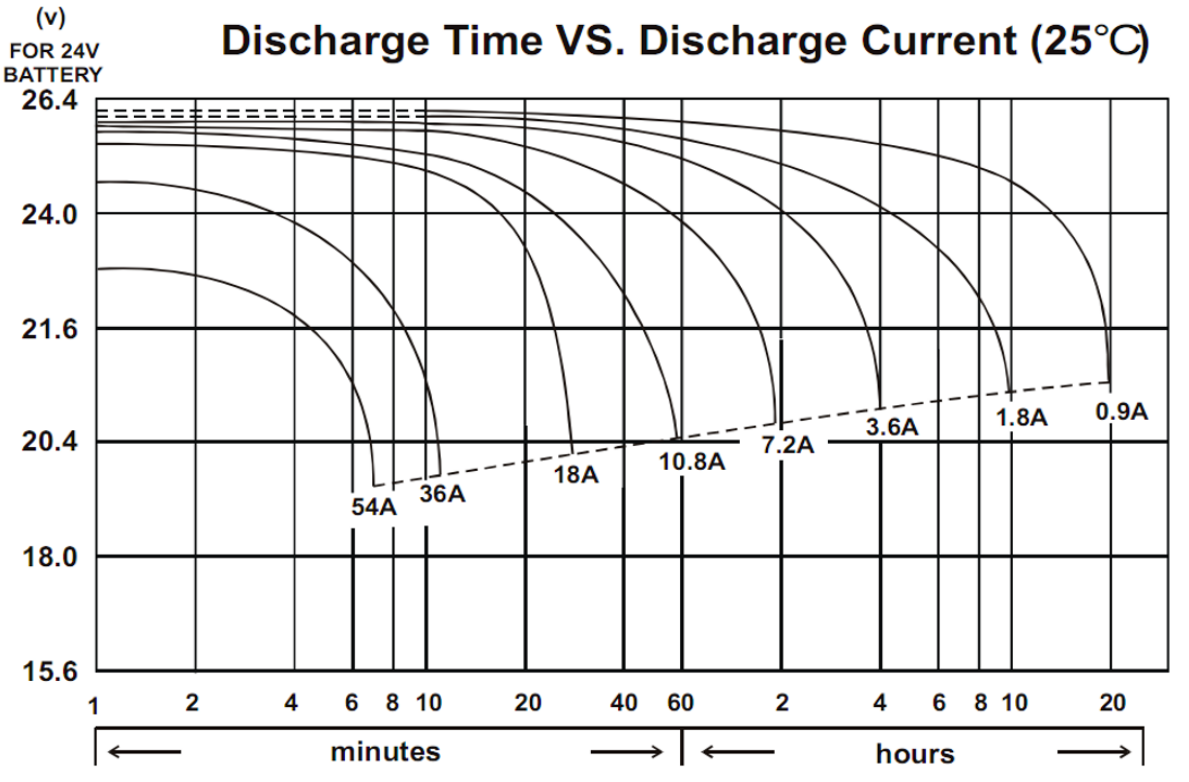
\includegraphics[width=9.2cm]{Pictures/EndladekuvenSLA.png}}
    \caption{Discharge time over different currents for the SLA battery of the Husky \cite[p.21]{SLAKurven}.}
    \label{fig:EndladekuvenSLA}
\end{figure}
With this curve, the SoC is estimated using the measured current and potential of the battery.
First of all, each curve has to be approximated. For this, a 4th degree polynomial is used.
It captures the curve fairly accurately within the usable range of the battery.
To simplify the estimation,  x- and y- data are flipped prior to the approximation.
This yields functions for different current dynamics that can be used to estimate the time of potential usage.
Comparing this value with the maximum time the battery can be used reveals the percentage of the battery which is already consumed.
\subsection{Validating the SoC estimation}
To validate the estimation, the battery  performs a complete discharge cycle. The  estimated SoC,  current, and  potential of the battery are recorded.
Fig. \ref{fig:SoCUeberZeit} shows the estimation of the SoC over one discharge cycle.
\begin{figure}[htbp]
    \centerline{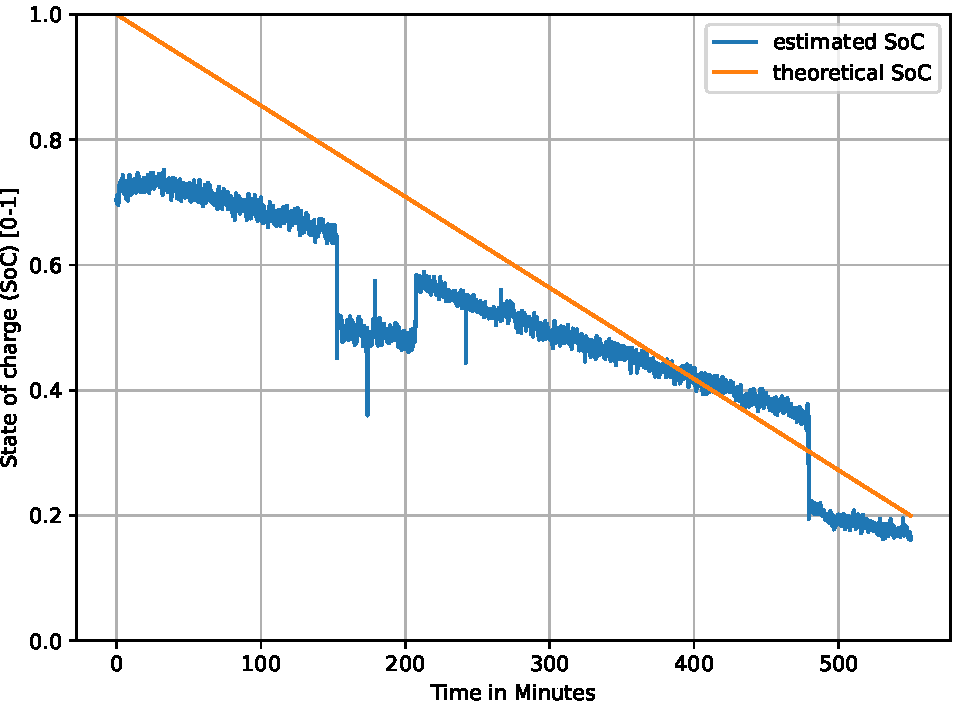
\includegraphics[width=9cm]{Pictures/SoCUeberZeit.pdf}}
    \caption{Comparison between the theoretical SoC and the estimated SoC over one discharge cycle.}
    \label{fig:SoCUeberZeit}
\end{figure}
As a further comparison, there is also the theoretical SoC calculated from the average current shown.
First of all, observe that the battery does not start at 100\%. Hence, it is likely that the battery does not hold a full charge anymore because of wear. The estimated SoC is a moving average over 100 values. However, there are some noises in  data.
A reason is that the measured potential and current are very noisy (Fig. \ref{fig:SpannungStromUeberZeit}).
\begin{figure}[htbp]
    \centerline{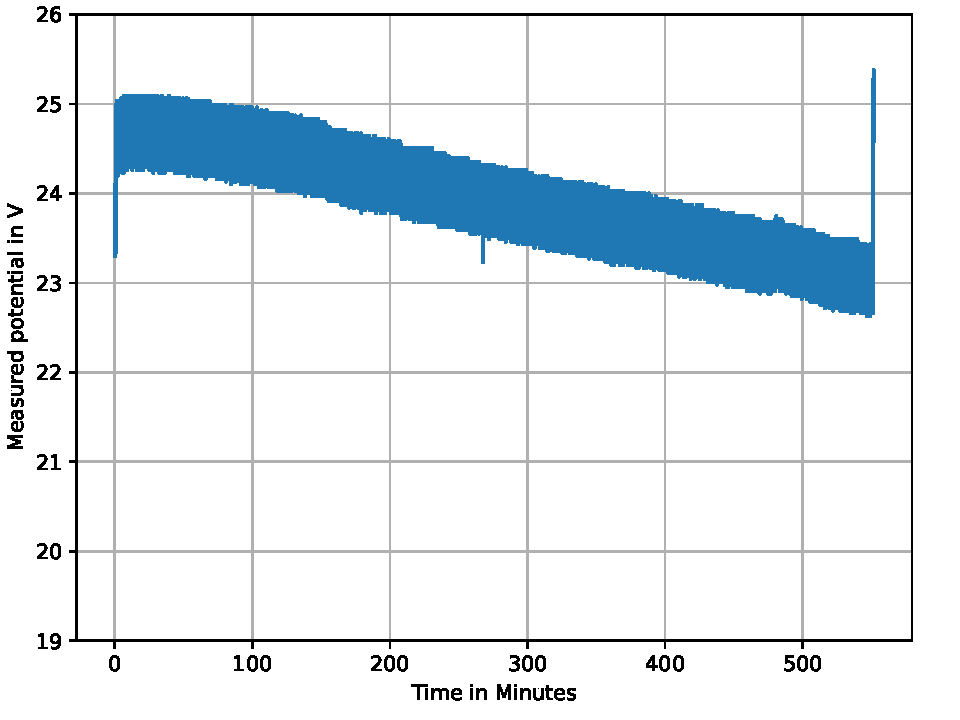
\includegraphics[width=4.5cm]{Pictures/SpannungUeberZeit.pdf}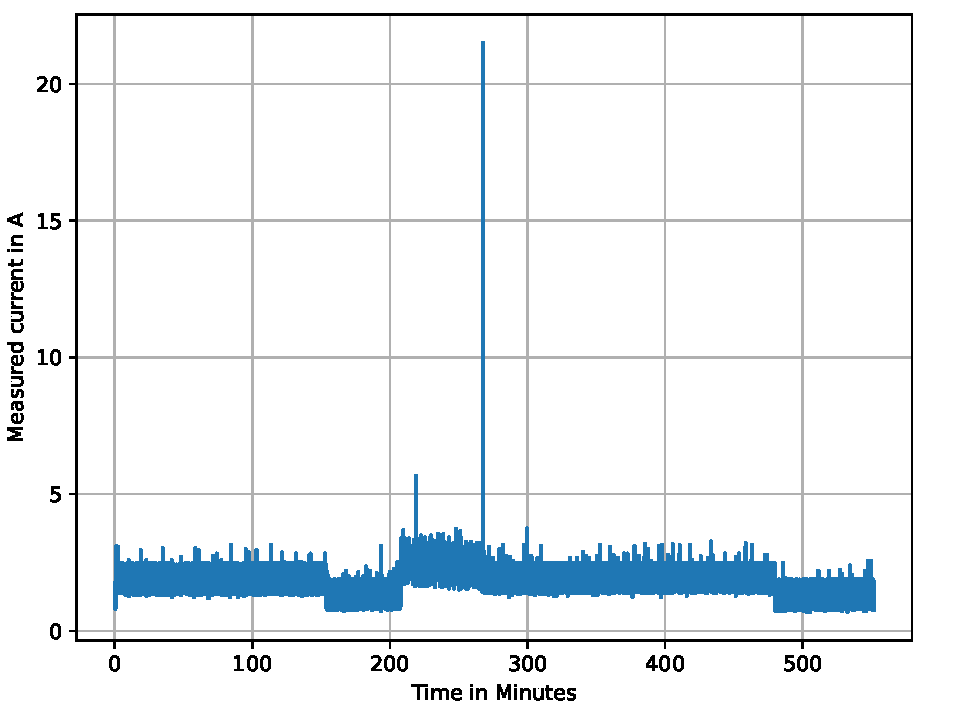
\includegraphics[width=4.5cm]{Pictures/StormUeberZeit.pdf}}
    \caption{Measured potential (l.h.s) and current (r.h.s) over one discharge cycle of the Husky battery.}
    \label{fig:SpannungStromUeberZeit}
\end{figure}
There are also big spikes in  data at around 150, 210 and 480 min.
At the same time, there are spikes in the current but not in the potential.
It is therefore likely that this is due to poor measurements.
At 270 min, there is  a big spike in the current. However, because there is also a spike in the potential of the battery, the  SoC hardly changes.
We did not find any document about the use of the sensor by Clearpath or how the measurements are made for the sake of replication.
But the new SoC estimation is much more precise than the old one and an underestimation of the SoC leads to an bigger safety margin which is also useful.
\section{Digital twin}
Digital twins developed within the cope of this work are built using Isaac Sim as part of the NVIDIA Omniverse. Isaac Sim works with USD, an open Universal Scene Description for 3D worlds, as information model. Native tools exist  to convert other information models, such as URDF, to USD. Hence, most scenarios involving third-party models can be  imported. To connect to the OPC-UA server of a DC, a client is needed. This is implemented via an extension for Isaac Sim.
\subsubsection{Composition and decomposition}
In certain applications, such as testing and verification in co-working and co-innovation for product development, data related to a critical system part of a system of systems might be sensitive and the access to them is prohibited.  DCs allows for directly selecting one or many targeted systems from  decentralized pools of systems offering open data to assemble and experiment different configuration of their digital twins even remotely. Similarly, each  DC can be shut down, which implicitly  indicates a transactional end-of-life of a related digital twin,  leading to its removal from the distributed system of digital twin systems.  %and seamlessly restricting the collection to different parts offering open data to experiment digital twins of associate part.
%	To reflect the modularity of the robot system and the decentralized network approach, multiple different configurations of the robot system are created.
%The extension has an Graphical User Interface (GUI) in which the configuration of the robot system can be chosen.

%Regardless of the selected configuration, clients can choose to which OPC-UA server they want to connect.
\subsubsection{Tests driven by hybrid data}
As composition involves measured data from physical systems, a remote system of digital twin systems might be assembled using models driven by simulation-generated data. This allows to test scenarios with desired boundary conditions. 
For example, it can be predicted if the Husky (synthetic data) will tip over when the Kinova (measured data) arm performs a \mbox{specific movement, long before the Husky is bought.}
%For that, a configuration with the Husky and a Kinova arm is loaded and a connection is established to the physical robot.
%The Kinova arm can now be moved with the controller and  any movement can be tested.\\
\subsection{Robot control based upon joint states of the digital twin}
Current joint states of a digital twin of a robot can be exposed using its associated DC and tracked by the corresponding physical surrogate acting as a client, as done in \cite{kaigom2020value}.
\subsection{Location-agnostic monitoring of selected systems of systems of systems}
%Furthermore it is possible to open a graph in which  data on the robot are displayed.
%So the 
Non-visible robot data like  current or temperature of the robot joints can be visualized using virtual cues.
Even if some  robots are not physically part of robotized system of systems but distributed instead, it is still possible to select and connect to a targeted robot and monitor its states  e.g. in the globally accessible Metaverse (e.g., the Omniverse of NVIDIA) \cite{kaigom2023metarobotics}.
%To make the digital twin more realistic you can choose in the GUI to load a 3D scan of the university as an environment for the digital twin (Fig. \ref{fig:CompareDigitalReal}).
\begin{figure}[t]
    \centerline{\includegraphics[height=3cm]{Pictures/DigitalerTwinNachgestellt1.JPG}\hspace{0.1cm}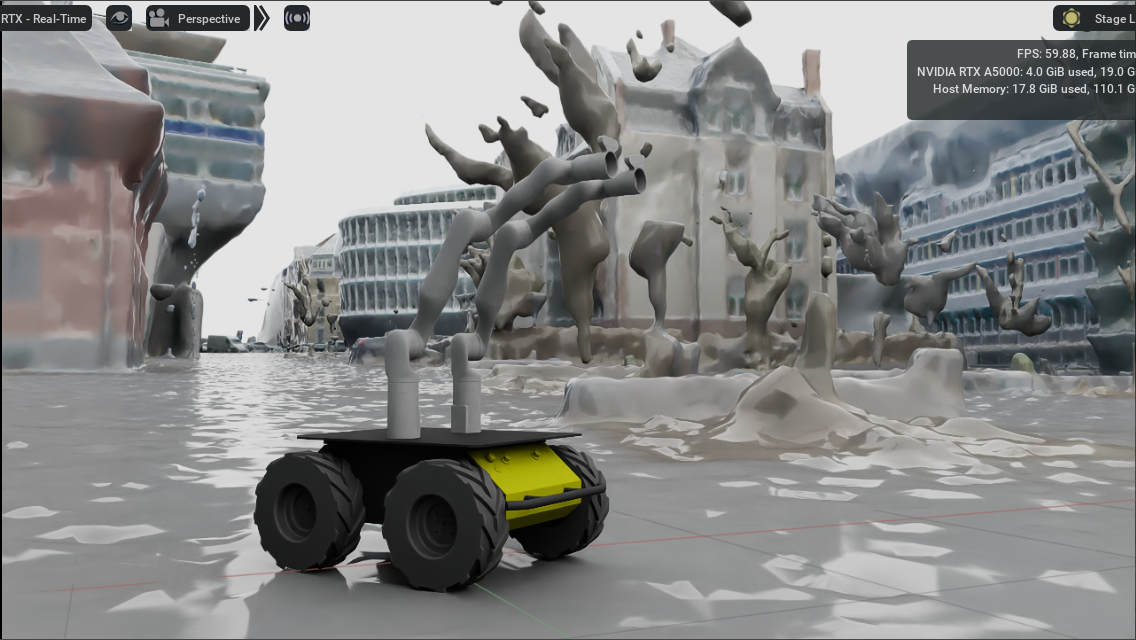
\includegraphics[height=3cm]{Pictures/DigitalerTwinNachgestellt2.png}}
    \caption{Comparison of the digital twin (l.h.s) and the real robot (r.h.s).}
    \label{fig:CompareDigitalReal}
\end{figure}

\section{Remote access}
 To monitor  robotic systems of digital twin and physical systems from everywhere, as in $\pi$-HRC introduced in \cite{kaigom2023metarobotics}, a remote access to the DC is necessary.
A mobile 5G router is mounted on the Husky. All DCs are connected to this router with Virtual Private Network (VPN) capabilities harnessed by  clients for secure tunneling. 
Figures \ref{fig:RemoteAccess} and \ref{fig:AufbauBilder} show how different clients (i.e., notebook, mobile phone) have access to the battery state of the Husky in the Lab \textit{from a train in motion in dense city traffics}, as pursued by Metarobotics \cite{kaigom2023metarobotics}.
\begin{figure}[htbp]
    \centerline{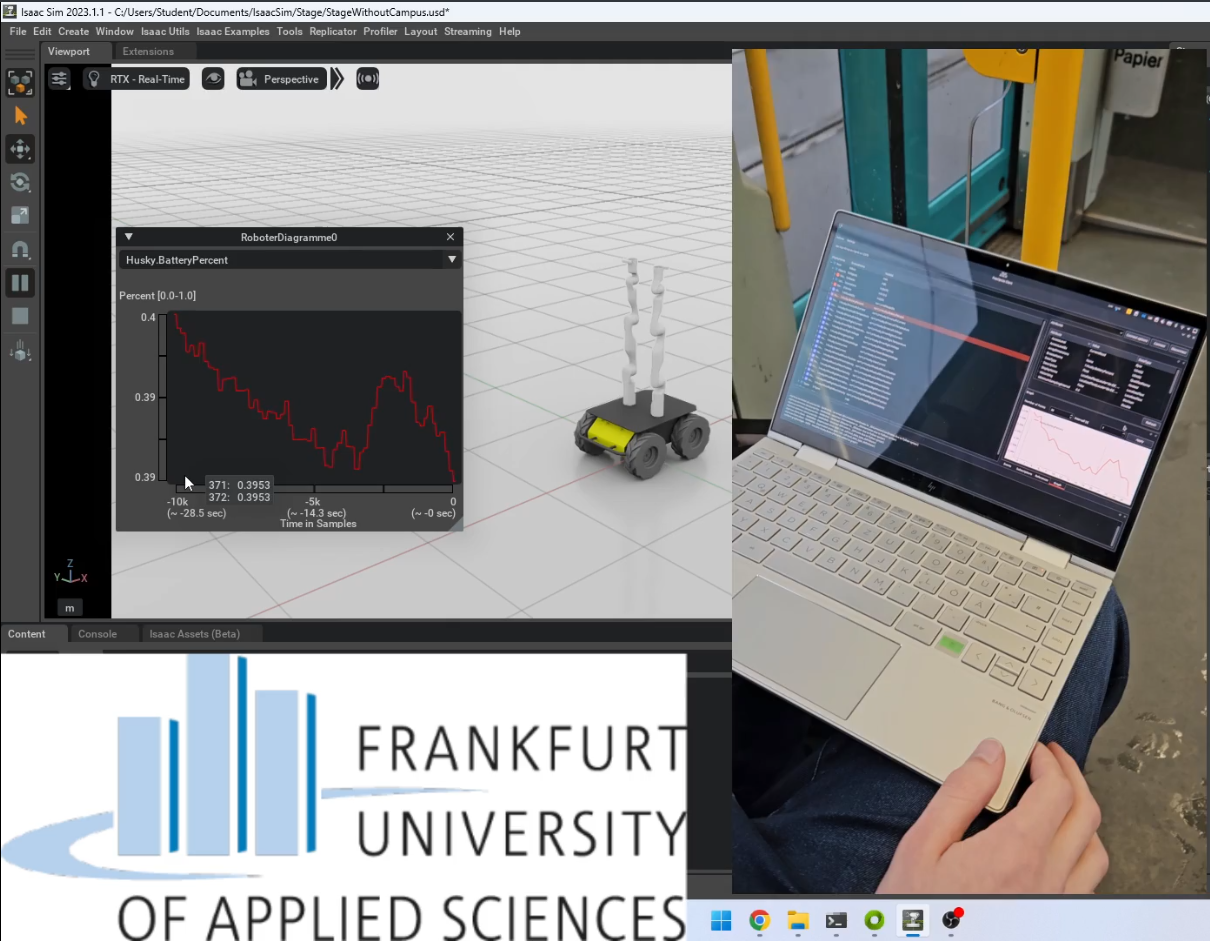
\includegraphics[width=8.9cm]{Pictures/ZugZugriff.png}}
    \caption{Example of the low-latency remote access to the DC of the robot in the university lab from a train moving in a massively dense city traffics.}
    \label{fig:RemoteAccess}
\end{figure}
For that, a special Sim Card for the router is needed.
It requires a public IP-Address. %This is currently not a typical usage for Sim Cards.
%Normally they get their Messages like push notification via a Google or Apple server.
%Without any public IP-Address, it is currently not possible to reach the VPN server.
As an alternative, a software like ngrok can be used  to make a tunnel to the DC. Hence, no public IP-Address is \mbox{needed but for each DC a separate tunnel is required.}
\section{Discussion}
Compared to the network that was built in \cite{SotaCAN}, the OPC-UA standard appears to deliver versatile connectivity capabilities when it comes to support information exchanges in evolving systems of hybrid systems in different contexts at the same time. Developed and employed DC components enable the  semantic integration and  seamless reconfiguration of such robotized systems even in motion to complete manipulation or relocation tasks. Plug, Move, and Automate (PMA) is therefore an added value of DCs. Their synchronization can be further enhanced in terms of privacy using smart contract-based transactions. A blockchained traceability of the metamorphosis of systems of hybrid systems at e.g. the structure, data, knowledge, as well as generative and collective intelligence are likely to elevate the \mbox{performance of DC-driven systems of systems.}

\begin{figure}[b]
	\centerline{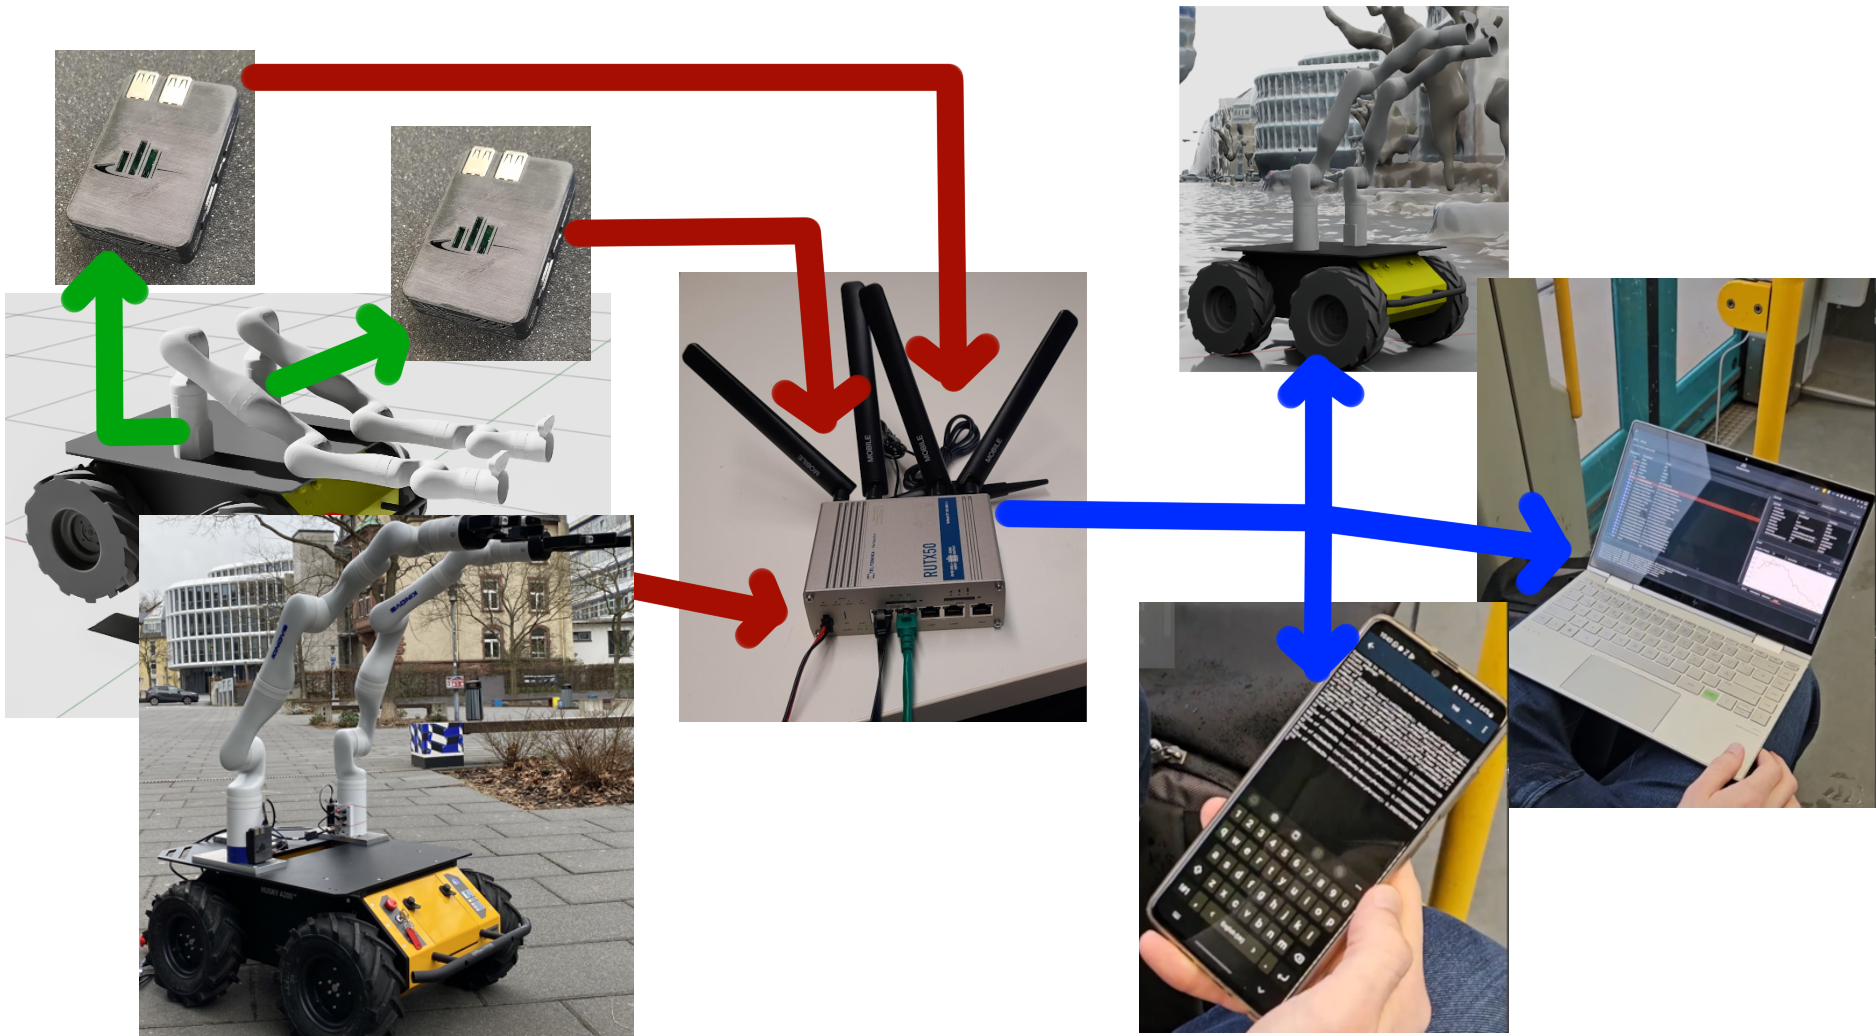
\includegraphics[width=8.9cm]{Pictures/AufbauBilder.png}}
	\caption{Visualization of the data structure using a real example.}
	\label{fig:AufbauBilder}
\end{figure}

%Furthermore, with the DC, it is possible to integrate different distributed robotied systems in the same network.This is also an advantage, when compared with \cite{SotaROS} because the robots do not need to be able to communicate via ROS. Indeed, the DC translates between the robot and the large network of decentralized hybrid devices.The interoperability between ROS and OPC-UA from \cite{StoaROStoOPCUA} is extended with the data connector.
%With the Kortex API a second communication standard is added and extendability for even more standards is easily provided.Q
%The middleware from \cite{SotaFusion} is proprietary and provides no further features over OPC-UA.
%The most similar is \cite{SotaRaconteur} due to it is an open source middleware.
%While OPC-UA is an industry standard, Robot Raconteur is lesser known.
\section{Conclusion}
This work has described the development of DCs that enable the dynamic formation of a network of loosely coupled, decentralized, semantically interoperating, and moving systems.  This has been done using the OPC-UA standard (Fig. \ref{fig:AufbauBilder}) to unify the information exchange between any virtual and physical OPC UA capable device, a ROS-, and a Kortex API-driven robot. The loose coupling facilitates the reconfiguration of systems of systems. Unlike monolithic approaches, DCs enable the modular and remote access to  single hybrid devices that constitute the system of systems even in motion. The effectiveness of the approach has been demonstrated in practice by successfully carrying out the remote monitoring of a mobile system of \mbox{robotic systems from the cabin of a moving train.}% in city traffics. 

%It is also possible to expand the data connector to work with many different robots from various manufacturers.
%The shown digital twin proves it is easy to connect to different robots when they are all using the same standard and the performance tests have shown this standard is fast enough to deliver a accurate digital twin model.
%Through the possibility of an remote connection to the different data connector is with this setup possible to monitor the robot system from all over the world.

\begin{thebibliography}{00}
	\bibitem{mbakop2023integrated}Mbakop, S., Tagne, G. \& Merzouki, R. Integrated Design Method for Systems of Systems: Application to the Autonomous Management of an Industry 4.0 Supply chain. {\em 2023 18th Annual System Of Systems Engineering Conference (SoSe)}. pp. 1-6 (2023)
\bibitem{SotaCAN}Chan, K.W., Mahyuddin, M.N., Khoo, B.E. (2021). Network-Based Cooperative Synchronization Control of 3 Articulated Robotic Arms for Industry 4.0 Application. In: Md Zain, Z., et al. Proceedings of the 11th National Technical Seminar on Unmanned System Technology 2019 . NUSYS 2019. Lecture Notes in Electrical Engineering, vol 666. Springer, Singapore. https://doi.org/10.1007/978-981-15-5281-6\_30
\bibitem{SotaROS}U. U. S. K. Rajapaksha, C. Jayawardena and B. A. MacDonald, "ROS Based Heterogeneous Multiple Robots Control Using High Level User Instructions," TENCON 2021 - 2021 IEEE Region 10 Conference (TENCON), Auckland, New Zealand, 2021, pp. 163-168, doi: 10.1109/TENCON54134.2021.9707460.
\bibitem{StoaROStoOPCUA}A. Tripathy, J. van Deventer, C. Paniagua and J. Delsing, "Interoperability Between ROS and OPC UA: A Local Cloud-Based Approach," 2022 IEEE 5th International Conference on Industrial Cyber-Physical Systems (ICPS), Coventry, United Kingdom, 2022, pp. 1-5, doi: 10.1109/ICPS51978.2022.9816962.
\bibitem{SotaRaconteur}J. D. Wason and J. T. Wen, "Robot Raconteur®: Updates on an Open Source Interoperable Middleware for Robotics," 2023 IEEE 19th International Conference on Automation Science and Engineering (CASE), Auckland, New Zealand, 2023, pp. 1-8, doi: 10.1109/CASE56687.2023.10260569.
\bibitem{SotaFusion}Caliskanelli I, Goodliffe M, Whiffin C, Xymitoulias M, Whittaker E, Verma S, Skilton R. Engineering Interoperable, Plug-and-Play, Distributed, Robotic Control Systems for Futureproof Fusion Power Plants. Robotics. 2021; 10(3):108. https://doi.org/10.3390/robotics10030108
\bibitem{Industry4}Lasi, H., Fettke, P., Kemper, HG. et al. Industry 4.0. Bus Inf Syst Eng 6, 239–242 (2014). https://doi.org/10.1007/s12599-014-0334-4
\bibitem{CommTechnology} P. Marcon et al., "Communication technology for industry 4.0," 2017 Progress In Electromagnetics Research Symposium - Spring (PIERS), St. Petersburg, Russia, 2017, pp. 1694-1697, doi: 10.1109/PIERS.2017.8262021.
\bibitem{OPCUA}Open Platform Communication Foundation, Unified Architecture, https://opcfoundation.org/about/opc-technologies/opc-ua/, last checked 09.02.2024.
\bibitem{CommunicationCommarison} Profanter, Stefan, Tekat, Ayhun, Dorofeev, Kirill, Rickert, Markus, Knoll, Alois. (2019). OPC UA versus ROS, DDS, and MQTT: Performance Evaluation of Industry 4.0 Protocols. 10.1109/ICIT.2019.8755050. 
\bibitem{open62541}Florian Palm, Sten Gruner, Julius Pfrommer, Markus Graube, Leon Urbas, open62541 – der offene OPC UA Stack, https://publica-rest.fraunhofer.de/server/api/core/bitstreams/d860fd4c-c051-4e71-815b-23c7fc4c2549/content
\bibitem{ComparOPCUAPaper}Mühlbauer, Nikolas; Kirdan, Erkin; Pahl, Marc-Oliver; Waedt, Karl (2021): Feature-based Comparison of Open Source OPC-UA Implementations. INFORMATIK 2020. DOI: 10.18420/inf2020\_34. Gesellschaft für Informatik, Bonn. PISSN: 1617-5468. ISBN: 978-3-88579-701-2. pp. 367-377. 5th GI/ACM I4.0 Standardization Workshop on Industrial Automation and Control Systems. Karlsruhe. 28. 09. - 2. 10. 2020
\bibitem{KortexUDP} Kinova Robotics Inc., Kortex TransportClient classes, https://docs.\\kinovarobotics.com/kortex/linked\_md/cpp\_transport\_router\_session\_\\notif.html\#transportclient-classes, last checked 08.02.2024.
\bibitem{SLAKurven} Clearpath. Husky A200 UGV User Manual. url: https://clearpathrobotics.com/husky-documentation/ last checked 21. 10. 2023.
\bibitem{kaigom2020value}Guiffo Kaigom, E. \& Roßmann, J. Value-driven robotic digital twins in cyber–physical applications. {\em IEEE Transactions On Industrial Informatics}. \textbf{17}, 3609-3619 (2020)
\bibitem{kaigom2023metarobotics}Guiffo Kaigom, E. Metarobotics for Industry and Society: Vision, Technologies, and Opportunities. {\em IEEE Transactions On Industrial Informatics}. (2023)
\end{thebibliography}
\end{document}